\documentclass[12pt]{article}
\usepackage{listings}
\usepackage{textcomp}
\usepackage{hyperref}
\usepackage{graphicx}
\usepackage{float}
% LaTeX settings for MATLAB code listings
% based on Ted Pavlic's settings in http://links.tedpavlic.com/ascii/homework_new_tex.ascii
\usepackage{listings}
\usepackage[usenames,dvipsnames]{color}

% This is the color used for MATLAB comments below
\definecolor{MyDarkGreen}{rgb}{0.0,0.4,0.0}

% For faster processing, load Matlab syntax for listings
\lstloadlanguages{Matlab}%
\lstset{language=Matlab,                        % Use MATLAB
        frame=single,                           % Single frame around code
        basicstyle=\small\ttfamily,             % Use small true type font
        keywordstyle=[1]\color{Blue}\bfseries,        % MATLAB functions bold and blue
        keywordstyle=[2]\color{Purple},         % MATLAB function arguments purple
        keywordstyle=[3]\color{Blue}\underbar,  % User functions underlined and blue
        identifierstyle=,                       % Nothing special about identifiers
                                                % Comments small dark green courier
        commentstyle=\usefont{T1}{pcr}{m}{sl}\color{MyDarkGreen}\small,
        stringstyle=\color{Purple},             % Strings are purple
        showstringspaces=false,                 % Don't put marks in string spaces
        tabsize=5,                              % 5 spaces per tab
        %
        %%% Put standard MATLAB functions not included in the default
        %%% language here
        morekeywords={xlim,ylim,var,alpha,factorial,poissrnd,normpdf,normcdf},
        %
        %%% Put MATLAB function parameters here
        morekeywords=[2]{on, off, interp},
        %
        %%% Put user defined functions here
        morekeywords=[3]{FindESS, homework_example},
        %
        morecomment=[l][\color{Blue}]{...},     % Line continuation (...) like blue comment
        numbers=left,                           % Line numbers on left
        firstnumber=1,                          % Line numbers start with line 1
        numberstyle=\tiny\color{Blue},          % Line numbers are blue
        stepnumber=5                            % Line numbers go in steps of 5
        }

% Includes a MATLAB script.
% The first parameter is the label, which also is the name of the script
%   without the .m.
% The second parameter is the optional caption.
\newcommand{\matlabscript}[2]
  {\begin{itemize}\item[]\lstinputlisting[caption=#2,label=#1]{#1.m}\end{itemize}}

\setlength{\oddsidemargin}{0in}
\setlength{\evensidemargin}{0in}
\setlength{\textheight}{9in}
\setlength{\textwidth}{6.5in}
\setlength{\topmargin}{-0.5in}

\hypersetup{
    colorlinks=true,
    urlcolor=blue,
    filecolor=magenta,
}

%%%%%%%%%%%%%%%%%%%%%%%%%%%%%%%%%%%%%%%%%%%%%%%%%%%%%%%%%%%%%%%%%%%%%%%%%%%
\title{\bf Problem Set 1\\[2ex] 
       \rm\normalsize ECS 174 --- Spring 2020}
\date{\today}
\author{\bf Nikhil Razdan}

\begin{document}
\maketitle
%%%%%%%%%%%%%%%%%%%%%%%%%%%%%%%%%%%%%%%%%%%%%%%%%%%%%%%%%%%%%%%%%%%%%%%%%%%

\newpage
\section*{Short answer problems}
\subsection*{Problem 1}
\subsubsection*{Question}
Give an example of how one can exploit the associative property of convolution to more
efficiently filter an image.

\subsubsection*{Answer}
Using separability, we can apply a kxk mask onto an nxm matrix using less operations than without.

\noindent
For example, say we are applying a smoothening filter using a Gaussian mask. Lets say our mask is 4x4 and our image we are applying it to is 9x9. For each pixel, we have to apply our mask and multiply each of the surrounding pixels by the mask value. This would mean we have to do 16 multiplications (one for each element in our 4x4 mask), which means 16 or $k^2$ operations.

\noindent
Using separability, we can instead split our 4x4 mask into a 1x4 and 4x1 mask, such that these two masks multiplied by outer product give us our original mask. Then, in applying the masks to the appropriate pixels, we only have to 8, or $2k$ operations. This separation into two separate filters is only possible because the law of associativity applies. This means that it doesn't matter which order we apply the filters, we will get the same result. Mathematically, it is represented by $(f * g) * h = f * (g * h)$

\noindent
Let our matrix $M$ be:
\begin{table}[h!]
\begin{tabular}{|l|l|l|l|l|}
\hline
1  & 23 & 3  & 4  & 12 \\ \hline
1  & 3  & 2  & 23 & 12 \\ \hline
23 & 41 & 45 & 12 & 11 \\ \hline
1  & 54 & 3  & 43 & 4  \\ \hline
1  & 54 & 3  & 43 & 4  \\ \hline
\end{tabular}
\end{table}

\noindent
Let our filter $L$ be:
\begin{table}[h!]
\begin{tabular}{|l|l|l|l|l|}
\hline
0.0030 & 0.0133 & 0.0219 & 0.0133 & 0.0030 \\ \hline
0.0133 & 0.0596 & 0.0983 & 0.0596 & 0.0133 \\ \hline
0.0219 & 0.0983 & 0.1621 & 0.0983 & 0.0219 \\ \hline
0.0133 & 0.0596 & 0.0983 & 0.0596 & 0.0133 \\ \hline
0.0030 & 0.0133 & 0.0219 & 0.0133 & 0.0030 \\ \hline
\end{tabular}
\end{table}

\noindent
If we apply $L$ to $M(3,3)$, we get that $M'(3,3) = \sum_{r=1}^{r=5} \sum_{c=1}^{c=5} M(r,c) * L(r,c)$ \\
This involves $5 * 5 = 25 = k^2$ multiplications.

\noindent
If we instead find $R$ and $C$ such that $R \times C = M$, then apply $R$ to $M(:,3)$ then $C$ to the resulting matrix, we get $M'(3,3) = \sum_{c=1}^{c=5} C(c) * (\sum_{r=1}^{r=5} R(r) * M(r,:))(c)$ \\
This involves $5 + 5 = 10 = 2k$ multiplications.

\newpage
\subsection*{Problem 2}
\subsubsection*{Question}
This is the input image: [1 0 0 1 1 0 0 1]. What is the result of dilation with a structuring
element [1 1 1]?

\subsubsection*{Answer}
To compute dilation, we set all output pixels corresponding to the given structuring element to 1 if the current input pixel is 1.

Thus, when going through the pixels, we get the following steps, each new step corresponding to the next input pixel getting handled:

\begin{table}[h!]
\begin{tabular}{|l|l|l|l|l|l|l|l|}
\hline
- & - & - & - & - & - & - & - \\ \hline
\end{tabular}
\end{table}

\begin{table}[h!]
\begin{tabular}{|l|l|l|l|l|l|l|l|}
\hline
1 & 1 & - & - & - & - & - & - \\ \hline
\end{tabular}
\end{table}

\begin{table}[h!]
\begin{tabular}{|l|l|l|l|l|l|l|l|}
\hline
1 & 1 & - & - & - & - & - & - \\ \hline
\end{tabular}
\end{table}

\begin{table}[h!]
\begin{tabular}{|l|l|l|l|l|l|l|l|}
\hline
1 & 1 & 0 & - & - & - & - & - \\ \hline
\end{tabular}
\end{table}

\begin{table}[h!]
\begin{tabular}{|l|l|l|l|l|l|l|l|}
\hline
1 & 1 & 1 & 1 & 1 & - & - & - \\ \hline
\end{tabular}
\end{table}

\begin{table}[h!]
\begin{tabular}{|l|l|l|l|l|l|l|l|}
\hline
1 & 1 & 1 & 1 & 1 & 1 & - & - \\ \hline
\end{tabular}
\end{table}

\begin{table}[h!]
\begin{tabular}{|l|l|l|l|l|l|l|l|}
\hline
1 & 1 & 1 & 1 & 1 & 1 & - & - \\ \hline
\end{tabular}
\end{table}

\begin{table}[h!]
\begin{tabular}{|l|l|l|l|l|l|l|l|}
\hline
1 & 1 & 1 & 1 & 1 & 1 & 0 & - \\ \hline
\end{tabular}
\end{table}

\begin{table}[h!]
\begin{tabular}{|l|l|l|l|l|l|l|l|}
\hline
1 & 1 & 1 & 1 & 1 & 1 & 1 & 1 \\ \hline
\end{tabular}
\end{table}

\newpage
\subsection*{Problem 3}
\subsubsection*{Question}
Describe a possible flaw in the use of additive Gaussian noise to represent image noise.

\subsubsection*{Answer}
Additive Gaussian noise assumes that the noise is spread evenly and randomly within a specified variance based upon the Gaussian distribution. The "additive" part of the name means that we add the noise (whether positive or negative) to the existing image.

\noindent
This is a good model for random noise, such as the noise of electromagnetic interference in data traveling along links in the Internet. However, this is not a good way of modeling noise that follows under a specific pattern.

\noindent
For example, if you are on a phone call near a busy street, your phone will record all the audio, both the content of your voice and the noise of the street. If we want to clean up that noise and model it with additive Gaussian noise, we'd end up with a sub-optimal output. This is because the noise from a busy street has specific patters, namely that of cars driving past, producing a number of frequencies (via the Doppler effect), the speech of other humans (which only produces frequencies in a very particular wavelength), etc.

\noindent
In actuality, we do multiple passes of noise-reducing filters over the signal. The most important of the filters greatly reduces all the wavelengths above and below human speech, effectively leaving only the human speech remaining. Then, to remove noise from that signal, we could model the remaining noise in more complex ways. Additive Gaussian noise could be used at this point, but it is a naive way to model the noise produced.

\newpage
\section*{Programming problem: content-aware image resizing}
\subsection*{Problem 1}
Subplot of Images:
\begin{figure}[H]
  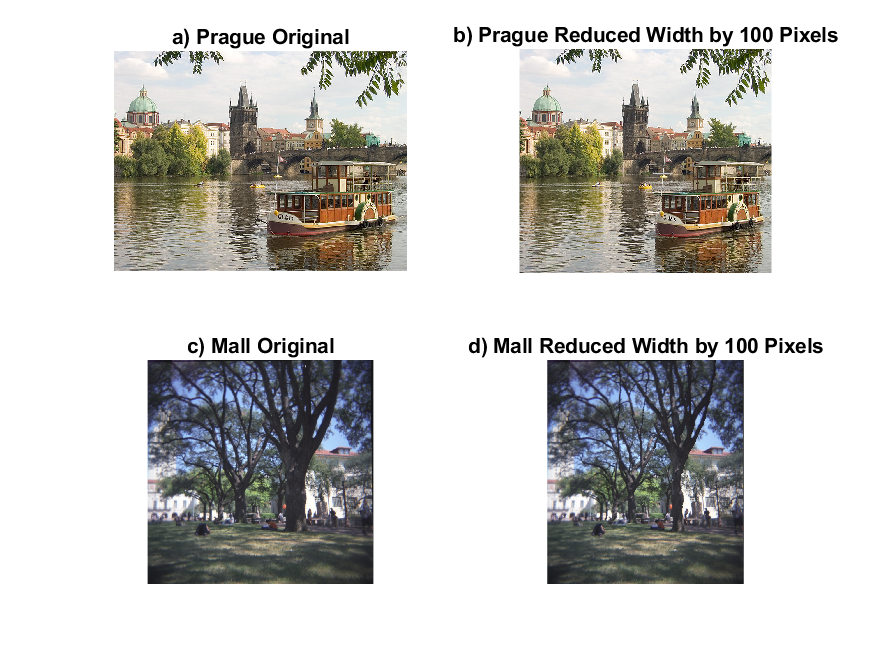
\includegraphics[width=\linewidth]{PS1_Q1.png}
  \label{fig:Subplot of Images}
\end{figure}

\noindent
Resized Prague Image:
\begin{figure}[H]
  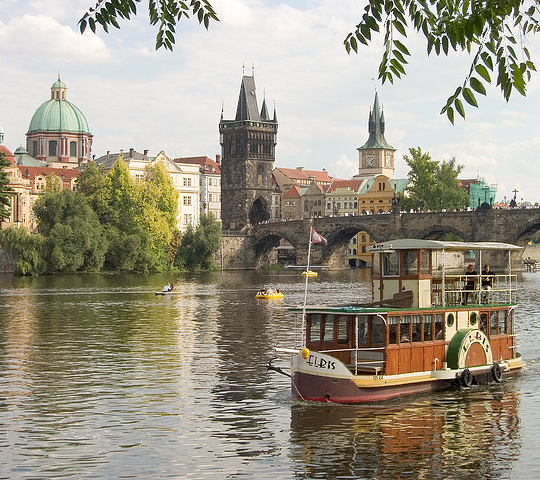
\includegraphics[width=100mm]{outputReduceWidthPrague.png}
  \label{fig:Resized Prague Image}
\end{figure}

\noindent
Resized Mall Image:
\begin{figure}[H]
  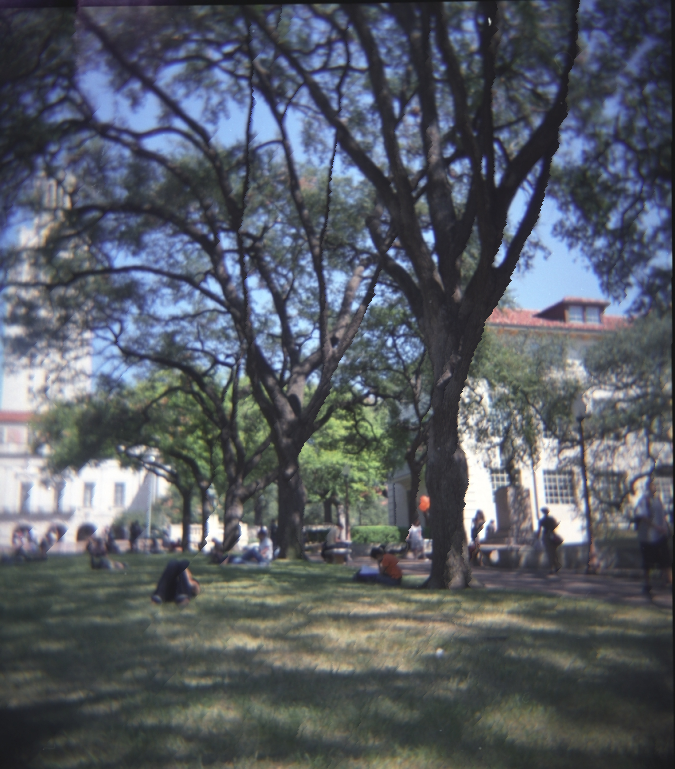
\includegraphics[width=100mm]{outputReduceWidthMall.png}
  \label{fig:Resized Mall Image}
\end{figure}

\newpage
\subsection*{Problem 2}
Subplot of Images:
\begin{figure}[H]
  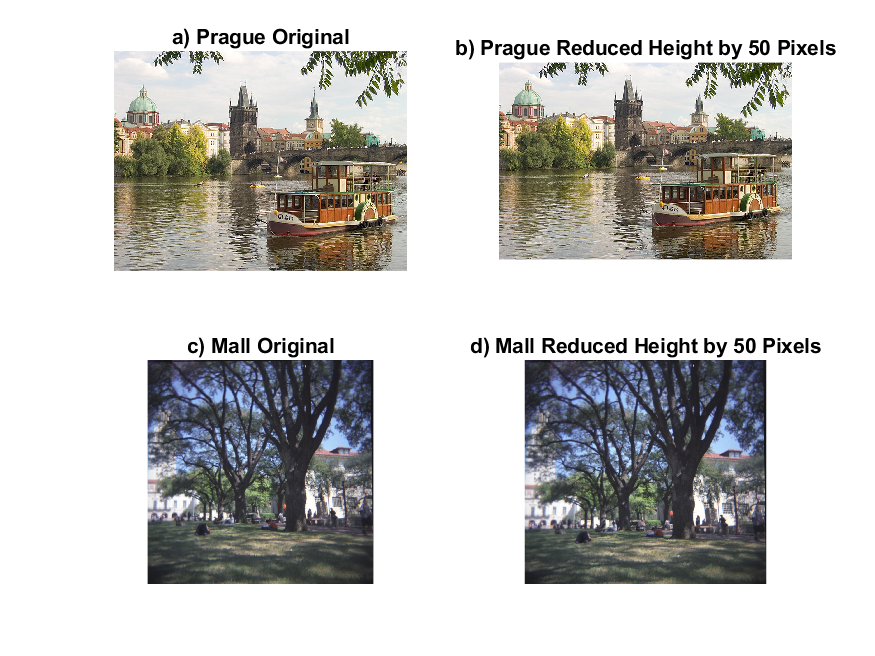
\includegraphics[width=\linewidth]{PS1_Q2.png}
  \label{fig:Subplot of Images}
\end{figure}

\noindent
Resized Prague Image:
\begin{figure}[H]
  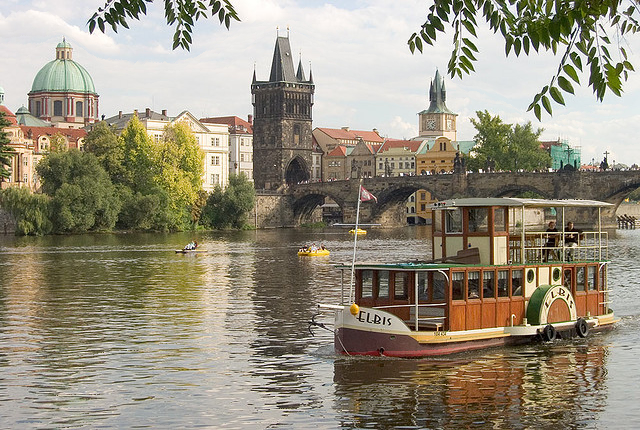
\includegraphics[width=100mm]{outputReduceHeightPrague.png}
  \label{fig:Resized Prague Image}
\end{figure}

\noindent
Resized Mall Image:
\begin{figure}[H]
  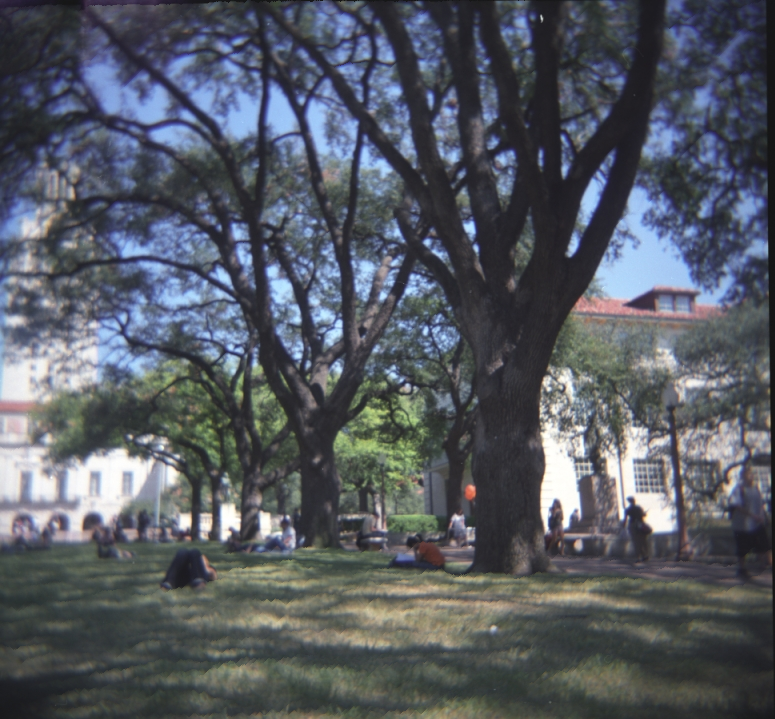
\includegraphics[width=100mm]{outputReduceHeightMall.png}
  \label{fig:Resized Mall Image}
\end{figure}

\newpage
\subsection*{Problem 3}
Energy Map:
\begin{figure}[H]
  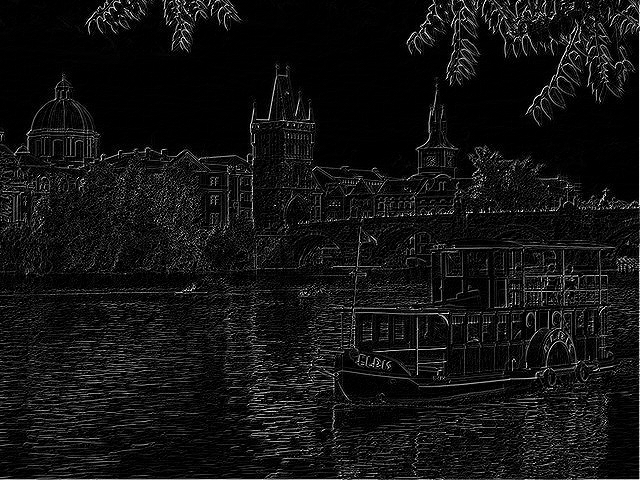
\includegraphics[width=100mm]{PS1_Q3_1.png}
\end{figure}

\noindent
Horizontal Cumulative Energy Map:
\begin{figure}[H]
  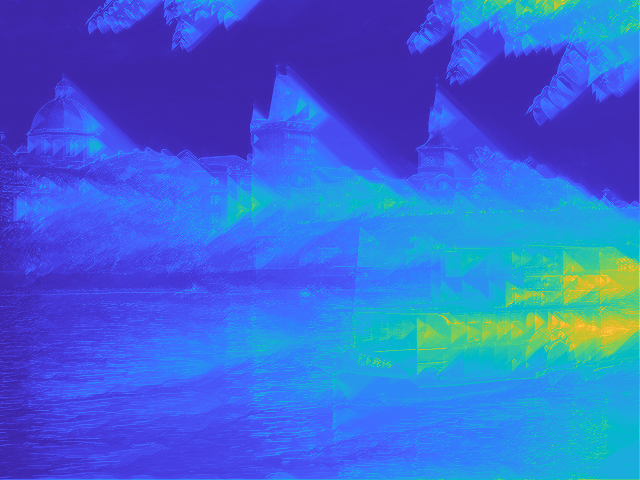
\includegraphics[width=100mm]{PS1_Q3_2.png}
\end{figure}

\noindent
Vertical Cumulative Energy Map:
\begin{figure}[H]
  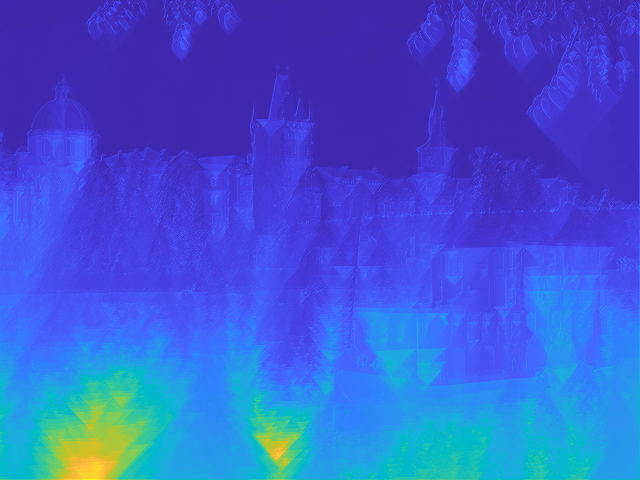
\includegraphics[width=100mm]{PS1_Q3_3.png}
\end{figure}

\noindent
The main thing to notice about the energy maps is how patches of information get swept along throughout the map. We can notice this especially in two places: with the leaves in the top right corner and with the boat in the bottom right corner. 

\noindent
With the leaves, we can see in the Vertical Cumulative Energy Map, that the intensities of the pixels below them begin large and then slowly taper off as there is more empty space. This is important because it shows how the Cumulative Energy Map slowly dies or builds as it traverses the Energy Map. This is what makes this seam carving algorithm so effective, as each pixel not only encodes its own importance in terms of the strength of the edge it creates, but also the importance of the other pixels that needed to be traversed to reach it.

\noindent
In terms of the differences between the horizontal and vertical map, this is most salient when looking at the boat in the bottom right corner. As we can tell, that area is much more important in the horizontal map than in the vertical. Why is this? Well, if we look at the image, we can see that the boat has a few columns of consistent pixels. In the body of the boat, there are sections which look essentially the same, but repeated. Whereas if we look by the rows, there is much more uniqueness, as there is the bottom of the boat touching the water, the body of the boat holding passengers, and the awning of the boat. This is how we can tell the differences in the different directions of the map. In one direction, we could have nearly infinite change, and in the other we could have 0.


\newpage
\subsection*{Problem 4}
Original Image:
\begin{figure}[H]
  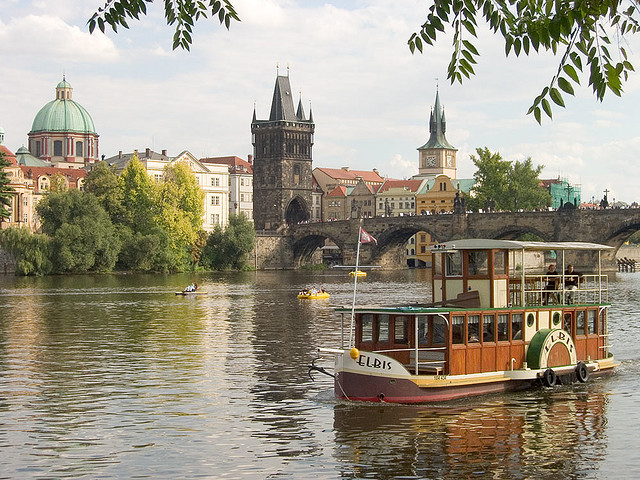
\includegraphics[width=100mm]{inputSeamCarvingPrague.jpg}
\end{figure}

\noindent
Horizontal Seam:
\begin{figure}[H]
  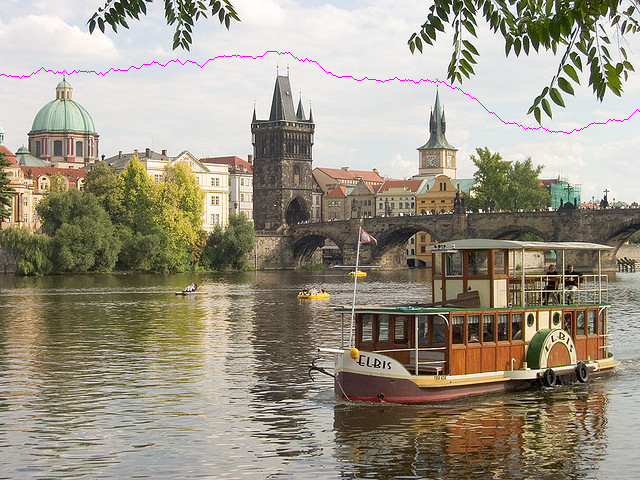
\includegraphics[width=100mm]{PS1_Q4_2.png}
\end{figure}

\noindent
Vertical Seam:
\begin{figure}[H]
  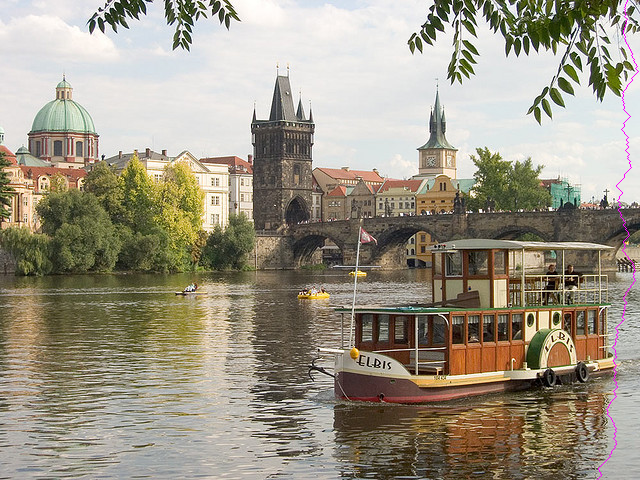
\includegraphics[width=100mm]{PS1_Q4_1.png}
\end{figure}

\noindent
These seams are the optimal because they take the past with the least cumulative energy, which means, essentially, that they pass through the least amount of edges, or rather the least important edges. We can see this using the energy maps from the previous question. In the first one, we see just the edges. It's clear why the horizontal seam is the optimal, as it just goes through almost completely empty space. But how about the vertical one? Well, this one is a little more complicated because it seems that there is vertical energy essentially everywhere. To figure this out, let's consult the Vertical Cumulative Energy Map, which shows that this seam importantly doesn't go through any of the high energy regions on the bottom left. If we spent time looking at each individual value, we could continue to reason that this seam minimizes the total energy we consume when traversing.

\newpage
\subsection*{Problem 5}
Original Image:
\begin{figure}[H]
  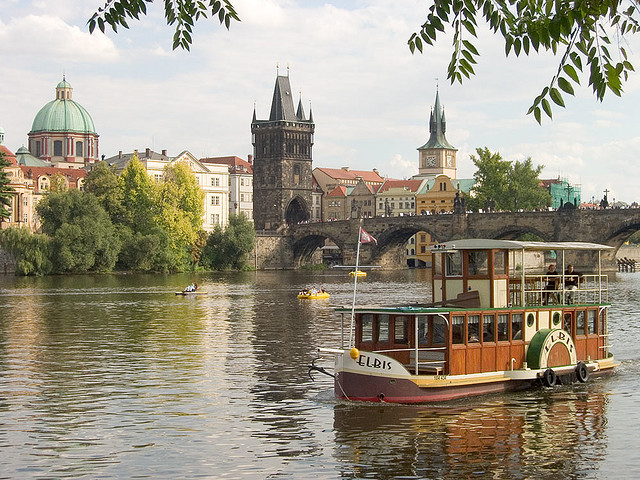
\includegraphics[width=100mm]{inputSeamCarvingPrague.jpg}
\end{figure}

\noindent
Horizontal Seam:
\begin{figure}[H]
  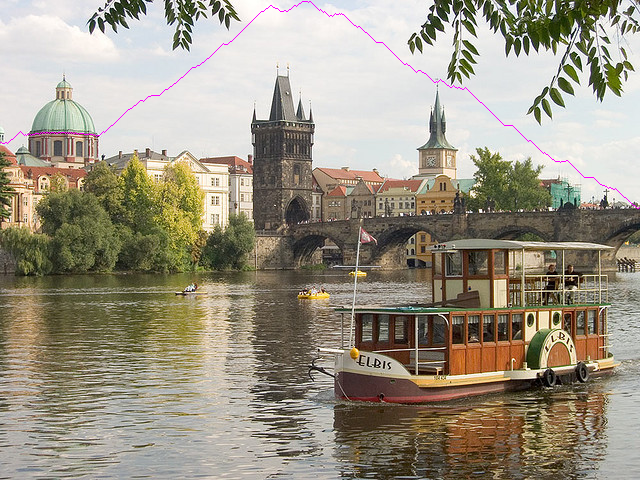
\includegraphics[width=100mm]{PS1_Q5_2.png}
\end{figure}

\noindent
Vertical Seam:
\begin{figure}[H]
  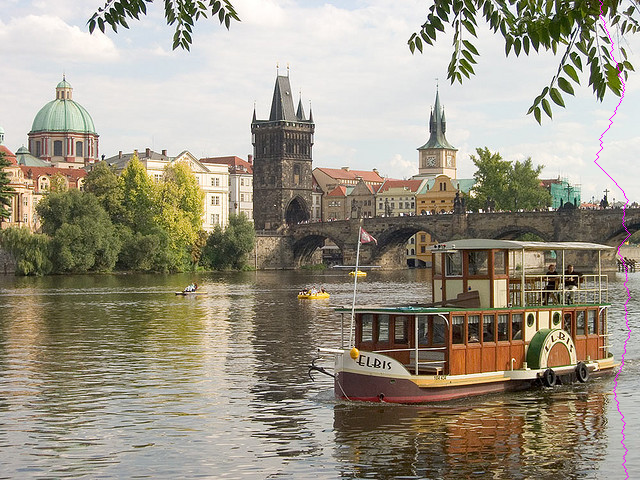
\includegraphics[width=100mm]{PS1_Q5_1.png}
\end{figure}

\noindent
In this example, we edited the energy function by changing out mask of our derivative. Instead of dx = [1, -1]; and dy [1; -1];, we have dx = [-0.5, 1, -0.5]; and dy [-0.5, 1; -0.5];.

\noindent
It's hard to predict exactly what the impact would be before applying it, but we can reason about a few things. We can see that it will make the derivative smoother in a way, as our range in the derivative larger. A derivative is supposed to utilize an infinitesimal range. Even the first equation we use is an approximation, which is necessary because our data is discrete instead of continuous. As such, this wider range will give us a less accurate answer, meaning our seams will be less optimal than our original energy function.

\newpage
\subsection*{Problem 6}
\subsubsection*{Test 1}
\textbf{a,b,c)}
\begin{figure}[H]
  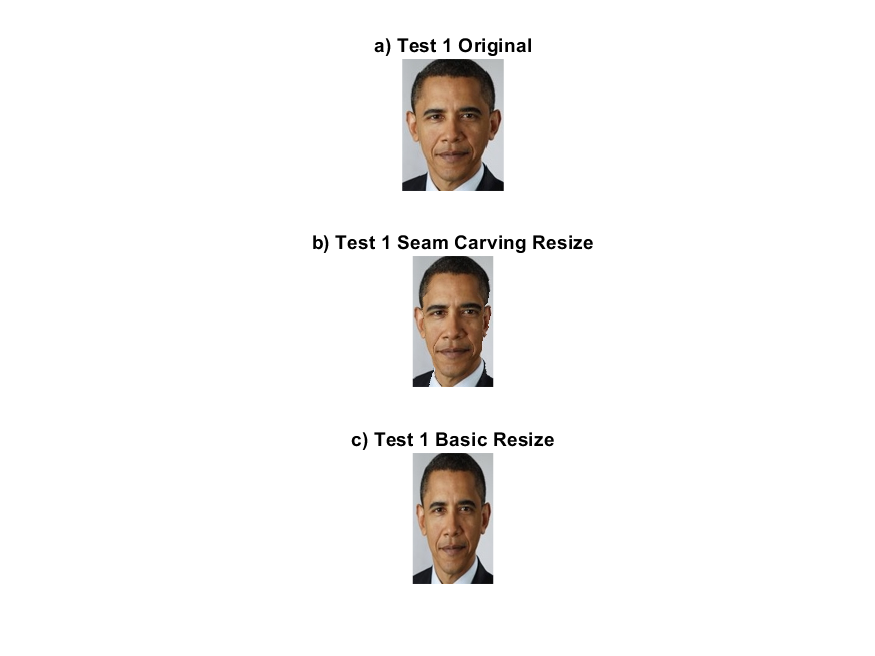
\includegraphics[width=\linewidth]{PS1_Q6_1.png}
\end{figure}

\noindent
\textbf{d)} \\
Original Image: 130 x 100 x 3 \\
Seam Carving Resize: 130 x 80 x 3 \\
Basic Resize: 130 x 80 x 3 \\

\noindent
\textbf{e)} \\
Continuous width decrement, 20 times in a row. \\

\noindent
\textbf{f)} \\
This image is used to test how seam carving fares with faces. There are three important things to notice about this image. \\
The first is how the important parts of the face, like the eyes and the mouth, are essentially preserved. This will be the case until most of the skin pixels of the face are removed, as a human face as a lot of empty space on it besides these essential features. This means, that in the early seam carvings, as with this example, the face is resized in a way that doesn't look too unnatural. However, this can have an adverse effect, which leads us to our next important point. \\
Humans are very sensitive to how faces look. The "empty space" as I called it before, like the forehead, is essential in how a person looks. Either too abnormally large or too abnormally small and a person looks \textit{off} in some way. This is important because seam carving will remove a lot of these "empty space" pixels first, leaving us with a face that looks alien. This can be seen in the example below, where we take the output seam carving image above and reduce the height by 40 pixels. The result is an ex-president who looks like he was squashed by an anvil in a children's cartoon.\\

\begin{figure}[H]
  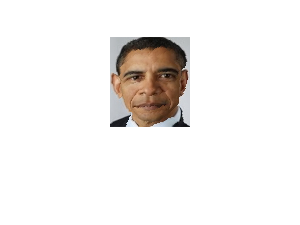
\includegraphics[width=\linewidth]{PS1_Q6_1_extra.png}
\end{figure}

\noindent
The third thing that is of note is the artifacts that develop in our example. This is a common problem with low-resolution images, but especially true with human faces. Again, this is an effect of human faces having a lot of content in the form of edges. Because there are so many strong edges, artifacts are more likely to develop and become even more apparent. 

\newpage
\subsubsection*{Test 2}
\textbf{a,b,c)}
\begin{figure}[H]
  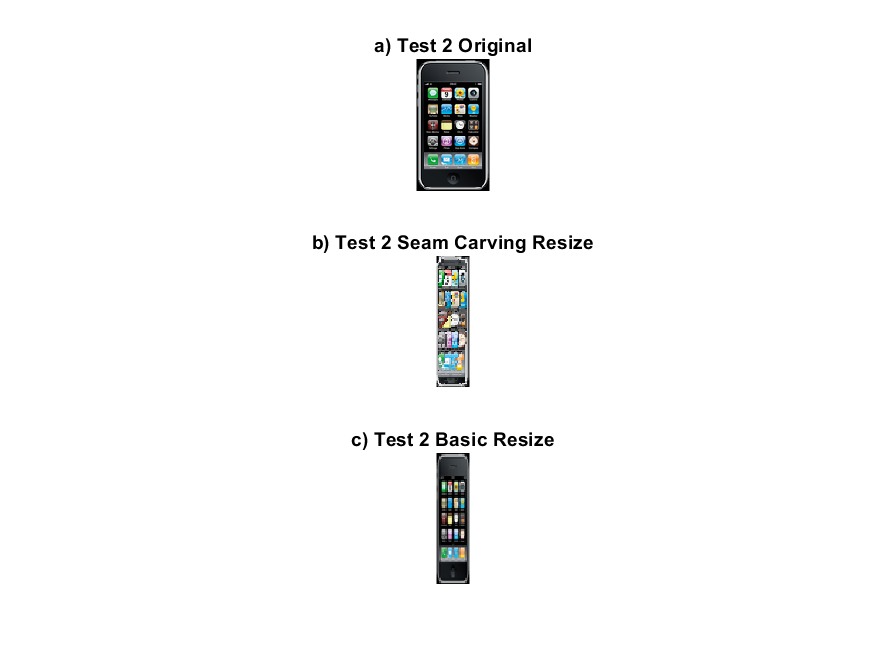
\includegraphics[width=\linewidth]{PS1_Q6_2.png}
\end{figure}

\noindent
\textbf{d)} \\
Original Image: 150 x 83 x 3 \\
Seam Carving Resize: 91 x 23 x 3 \\
Basic Resize: 91 x 23 x 3 \\

\noindent
\textbf{e)} \\
Continuous width decrement followed by height decrement, 59 times in a row. Extra one height decrement in beginning. \\

\noindent
\textbf{f)} \\
This example shows how seam carving preserves content in an image. Seam carving prioritizes pixels that store less edge information. As such, we can see that in this image, all the whitespace between the icons on the iPhone are removed. The icons are preserved because of the change in intensity of the image. One thing to note, however, is how our implementation of the algorithm works off a gray-scale image. This makes the algorithm much faster, but sacrifices some functionality of the seam carving resizing.

\newpage
\subsubsection*{Test 3}
\textbf{a,b,c)}
\begin{figure}[H]
  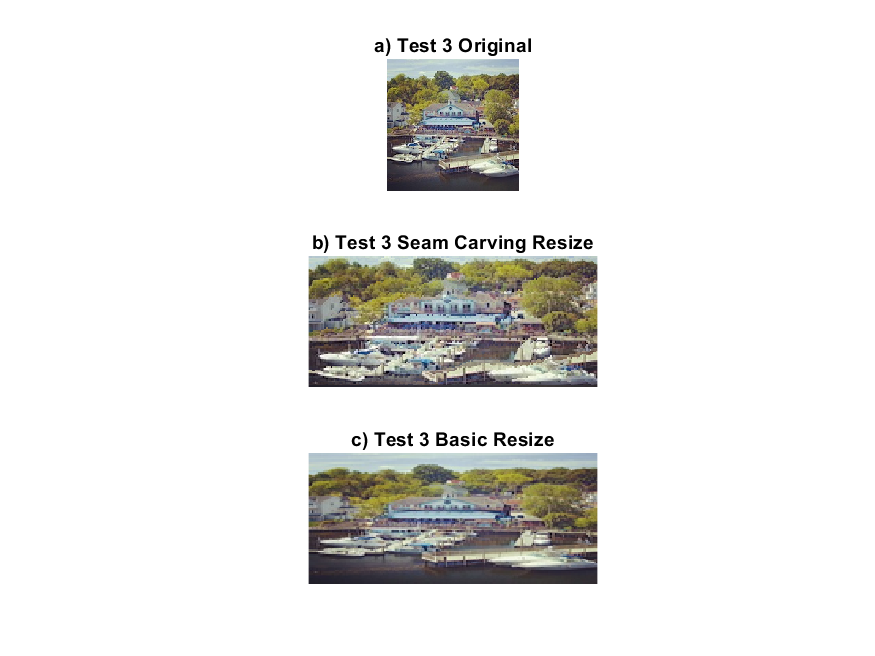
\includegraphics[width=\linewidth]{PS1_Q6_3.png}
\end{figure}

\noindent
\textbf{d)} \\
Original Image: 183 x 183 x 3 \\
Seam Carving Resize: 83 x 183 x 3 \\
Basic Resize: 83 x 183 x 3 \\

\noindent
\textbf{e)} \\
Continuous height decrement, 100 times in a row.

\noindent
\textbf{f)} \\
This image allows us to see clearly the advantages of context-aware resizing over basic resizing in terms of protecting the relative size of content in a busy image. There's not a lot of whitespace in the image and, because we remove more than half of the rows in the image, a good chunk of the information will be lost. However, we preserve most of the information in a way that it is still understandable. \\
This is especially useful when combined with image recognition and other more complex functions of computer vision that utilize machine learning. A lot of the challenge in making these algorithms useful in industry is making them less computationally taxing. However, by their very nature, with the amount of data they have to process, they take a lot of resources. Using seam carving, as seen in this example, we can greatly reduce the size of an image and still retain the key features. We, as humans, can still recognize the boats, the buildings, the trees, with less than half the data we originally were given. \\
Similarly, we could context-aware resizing to feed a machine learning agent data that is significantly reduced in size but still contains much of the relevant data. We could do this by removing pixels until all pixel values in the energy map were above some threshold, meaning they held some level of importance. Then, we would be left with only the important information to feed to the agent.

\end{document}
